% Options for packages loaded elsewhere
\PassOptionsToPackage{unicode}{hyperref}
\PassOptionsToPackage{hyphens}{url}
%
\documentclass[
  fleqn,ebook]{ic}
\usepackage{amsmath,amssymb}
\usepackage{lmodern}
\usepackage{ifxetex,ifluatex}
\ifnum 0\ifxetex 1\fi\ifluatex 1\fi=0 % if pdftex
  \usepackage[T1]{fontenc}
  \usepackage[utf8]{inputenc}
  \usepackage{textcomp} % provide euro and other symbols
\else % if luatex or xetex
  \usepackage{unicode-math}
  \defaultfontfeatures{Scale=MatchLowercase}
  \defaultfontfeatures[\rmfamily]{Ligatures=TeX,Scale=1}
\fi
% Use upquote if available, for straight quotes in verbatim environments
\IfFileExists{upquote.sty}{\usepackage{upquote}}{}
\IfFileExists{microtype.sty}{% use microtype if available
  \usepackage[]{microtype}
  \UseMicrotypeSet[protrusion]{basicmath} % disable protrusion for tt fonts
}{}
\makeatletter
\@ifundefined{KOMAClassName}{% if non-KOMA class
  \IfFileExists{parskip.sty}{%
    \usepackage{parskip}
  }{% else
    \setlength{\parindent}{0pt}
    \setlength{\parskip}{6pt plus 2pt minus 1pt}}
}{% if KOMA class
  \KOMAoptions{parskip=half}}
\makeatother
\usepackage{xcolor}
\IfFileExists{xurl.sty}{\usepackage{xurl}}{} % add URL line breaks if available
\IfFileExists{bookmark.sty}{\usepackage{bookmark}}{\usepackage{hyperref}}
\hypersetup{
  pdftitle={Análise Descritiva e Comparativa da Covid-19},
  pdfauthor={Guilherme Fernandes Castro de Oliveira},
  hidelinks,
  pdfcreator={LaTeX via pandoc}}
\urlstyle{same} % disable monospaced font for URLs
\usepackage{longtable,booktabs,array}
\usepackage{calc} % for calculating minipage widths
% Correct order of tables after \paragraph or \subparagraph
\usepackage{etoolbox}
\makeatletter
\patchcmd\longtable{\par}{\if@noskipsec\mbox{}\fi\par}{}{}
\makeatother
% Allow footnotes in longtable head/foot
\IfFileExists{footnotehyper.sty}{\usepackage{footnotehyper}}{\usepackage{footnote}}
\makesavenoteenv{longtable}
\usepackage{graphicx}
\makeatletter
\def\maxwidth{\ifdim\Gin@nat@width>\linewidth\linewidth\else\Gin@nat@width\fi}
\def\maxheight{\ifdim\Gin@nat@height>\textheight\textheight\else\Gin@nat@height\fi}
\makeatother
% Scale images if necessary, so that they will not overflow the page
% margins by default, and it is still possible to overwrite the defaults
% using explicit options in \includegraphics[width, height, ...]{}
\setkeys{Gin}{width=\maxwidth,height=\maxheight,keepaspectratio}
% Set default figure placement to htbp
\makeatletter
\def\fps@figure{htbp}
\makeatother
\setlength{\emergencystretch}{3em} % prevent overfull lines
\providecommand{\tightlist}{%
  \setlength{\itemsep}{0pt}\setlength{\parskip}{0pt}}
\setcounter{secnumdepth}{5}
\usepackage{booktabs}
\renewcommand\maketitle{}

% Coloque aqui os pacotes LaTeX que serão utilizados ---------------------------
\usepackage{multicol}
\usepackage{enumitem}
\usepackage{wrapfig}
\usepackage[format=hang,labelfont=normalfont]{subcaption}
\usepackage{longtable}
\usepackage{xfrac}
\newcommand{\MiKTeX}   {\textsc{MiK}\TeX}
\newcommand{\BibLaTeX} {\textsc{Bib}\LaTeX}
\newcommand{\TeXstudio}{\TeX\textsf{studio}}
\newcommand{\JabRef}   {\textsf{JabRef}}
\newcommand{\ThisClass}{\texttt{\getclass}}
\newcommand{\texfile}  {\texttt{TCC.tex}}
\newcommand{\bibfile}  {\texttt{tcc.bib}}
\usepackage{indentfirst}
\usepackage{url}
\setlength{\parindent}{0.5cm}
\usepackage{float}
\usepackage{graphics}
\usepackage{graphicx}

% Coloque aqui a data e o local da Banca do TCC --------------------------------
\day{31}
\month{07}
\year{2021}
\city{Florestal}
\state{Minas Gerais}
% Coloque aqui o nome dos Professores da Banca ---------------------------------
% Se for orientadora mude o comando \orientador para \orientadora --------------
% Se for coorientadora mude o comando \coorientador para \coorientadora --------
\board{Fernando de Souza Bastos}%
      {}%
      {}
\coorientador{}
\orientador{Fernando de Souza Bastos}
%%%%%%%%%%%%%%%%%%%%%%%%%%%%%%%%%%%%%%%%%%%%%%%%%%%%%%%%%%%%%%%%%%%%%%%%%%%%%%%%
\ifluatex
  \usepackage{selnolig}  % disable illegal ligatures
\fi
\usepackage[]{natbib}
\bibliographystyle{abbrvnat3}

\title{Análise Descritiva e Comparativa da Covid-19}
\author{Guilherme Fernandes Castro de Oliveira}
\date{Última atualização: 02/09/2021}

\begin{document}
\maketitle

\begin{acknowledgement}

  Aqui você deve colocar os agradecimentos. Por exemplo:
  
  Primeiramente queria agradecer ao meu orientador Fernando de Souza Bastos por
  sempre estar me ajudando em qual seja o assunto ou dificuldade, a aprender
  cada vez mais sobre o R e sua comunidade, e pela consideração que tem comigo e
  todos os seus alunos.
  
  Agradeço aos meus amigos que sempre me deixam pra cima nos momentos mais
  difíceis e que nunca abandonam quando preciso deles.

  Agradeço também a Júlia Letícia Gonçalves Martins na ajuda na escrita desse
  exemplo de TCC, e todo o apoio nos projetos da minha vida.
  
  Agradeço a todos que fizeram parte da minha vida e me ensinaram algo, sendo
  assim ajudaram nesse trabalho indiretamente.
  
  E agradeço a você que utilizará esse modelo pela consideração.

\end{acknowledgement}
\begin{Resumo}
  
  Aqui você deve colocar o seu resumo. Por exemplo:
  
  Até os dias atuais, o curso de Licenciatura em Matemática da UFV - Campus 
  Florestal possui um protótipo para escrita do Trabalho de Conclusão do Curso
  criado na linguagem LaTeX, elaborado pelo professor Luis Alberto D'Afonseca, 
  disponível no site da graduação. Embasado nesse modelo já existente, este novo
  modelo foi criado com o pacote Bookdown para que pudesse ser escrito não 
  somente em LaTeX, mas também nas linguagens citadas acima, com o diferencial 
  mais importante o R e seus pacotes.
  
  É válido ressaltar que este padrão pode ser utilizado não somente pelo curso
  de Licenciatura em Matemática - Campus Florestal, mas sim por todos os cursos
  dos campus da Universidade Federal de Viçosa.
  
  Espero que todos utilizem, consigam fazer o seu TCC e enfim recebam o tão
  desejado diploma.
  
\end{Resumo}
\begin{Abstract}
  
  Aqui você deve colocar o seu rusumo em inglês. Por exemplo:
  
  Until today, the Mathematics Degree course at UFV - Campus Florestal has a
  prototype for writing the Course Conclusion Paper created in LaTeX language,
  elaborated by professor Luis Alberto D'Afonseca, available on the graduation
  website. Based on this existing model, this new model was created with the
  Bookdown package so that it could be written only in LaTeX, but also in the
  languages mentioned above, with the differential most importantly R and its
  packages.
  
  It is worth noting that this standard can be used not only by the course in
  Mathematics - Campus Florestal, but for all courses campus of the Federal
  University of Viçosa.
  
  I hope you all use it, get your TCC and finally receive the so desired
  University Degree.
  
\end{Abstract}

\tableofcontents

\hypertarget{Intro}{%
\section{Introdução}\label{Intro}}

De acordo com \cite{Mahasem1547}, na década de 60, o virologista britânico David
Tyrrell realizava pesquisas sobre a gripe comum que tinha como objeto de estudo
lavagens nasais de voluntários. A equipe de Tyrrell também estudava outros
diferentes vírus, entre eles havia o vírus da hepatite, vírus da bronquite
infecciosa, vírus da gastroenterite transmitidos por suínos, entre outros. Certo
dia, juntamente com a equipe que liderava, Tyrrell recebeu uma amostra de um
paciente doente de um internato de Surray, sul de Londres. Essa amostra foi
testada em mais de 20 experimentos à procura de alguma doença já conhecida
como, influenza A, B ou C, pars-influenza 1, 2, 3 ou 4 ou o vírus sincicial
respiratório, mas nenhum foi encontrado. Eles descobriram um novo patógeno, que
provocava os sintomas de uma gripe comum, entretanto fracassaram em cultivá-lo
em cultura celular de rotina para o prosseguimento dos estudos.

De acordo com uma reportagem da \cite{almeidaBBC}, os estudos obtiveram
importantes avanços após a virologista escocesa June Almeida, convidada
a trabalhar na escola de medicina do hospital St.~Thomas, se juntar à se juntar
à equipe de Tyrrel. Tal convite motivado pelo reconhecimento de seu trabalho que
permitia visualizar melhor determinados vírus por meio do uso de anticorpos.
Utilizando sua metodologia de visualização, June foi a primeira a conseguir
visualizar a amostra do patógeno em estudo pela equipe de Tyrrel. Ela observou
que havia semelhança com daquela com outras amostras já estudadas por ela ao
longo de sua carreira. Posteriormente, June, juntamente com Tyrrel e Anthony
Peter Waterson, diretor do hospital, confirmaram que o patógeno era um virús e
o denominaram de B814. Ao perceberem que se tratava de um novo gênero de vírus e
que o mesmo possuía uma estrutura morfológica com a aparência semelhante a de
uma coroa, denominaram o mesmo de Coronavírus. Observem a \ref{fig:coroa}.

\begin{figure}[H]
    \centering
    \caption{Modelo de virião de Coronavírus.}
    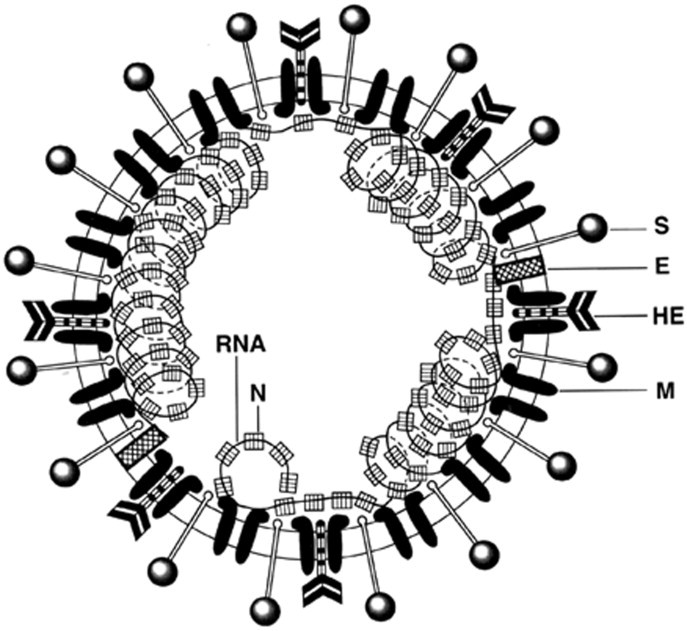
\includegraphics[width=6cm]{img/coroa.jpg}\\
    {\footnotesize \textbf{Fonte: }\cite{holmes1999coronaviruses}}
    \label{fig:coroa}
\end{figure}

Na mesma época, dos estudos de Tyrrel, outros pesquisadores estudando doenças
respiratórias similares, entre eles Dorothy Hamre e John J. Procknow, analisaram
amostras obtidas de estudantes de medicina com resfriado e relataram um tipo
semelhante de vírus que denominaram de 229E \citep{hamre1966new}. Outro pesquisador,
o doutor Kenneth McIntosh estava pesquisando sobre assuntos similares e
conseguiu isolar agentes sensíveis ao éter de outra amostra do sistema
respiratório humano, e por serem cultivados em cultura de órgãos foram
denominados de ``OC'' \citep{mcintosh1967recovery}. Após alguns anos, estudos
realizados por McIntosh, com técnicas sorológicas avançadas, resultaram em novas
informações sobre os surtos de coronavírus, por exemplo, ocorrem mais em
estações chuvosas, inverno e primavera do que no verão
\citep{mcintosh1970seroepidemiologic}. Entre os diferentes vírus da família corona os
que mais extensivamente foram estudados são o 229E e o OC43.

Após vários estudos epidemiológicos, de diferentes autores, citados no artigo
\cite{jahangir2020coronavirus}, os vírus da família Corona foram descobertos
associados a outras doenças já conhecidas pelos médicos, a maioria delas doenças
respiratórias como bronquite crônica, asma em adultos e idosos, a mais
predominante foi a pneumonia, em crianças e jovens adultos. O coronavírus não
infectam apenas humanos, mas também animais, com a velocidade e a quantidade que
esses casos apareciam em diversas espécies, camundongos, ratos, gatos, cães,
perus, galinhas, porcos e coelhos os estudos não se limitaram apenas as doenças
do sistema respiratório, mas também, a encefalite, hepatite e a gastroenterite.
Com base em estudos tanto genéticos e antigênicos, foi possível categorizar os
coronavírus tanto humanos quanto animais em 3 grandes divisões, observadas na
tabela \ref{tab:corona3div}, retirada do artigo \cite{jahangir2020coronavirus}.

\begin{table}[H]
    \centering
    \caption{Tabela categorizando os coronavírus.}
    \begin{tabular}{|c|p{5cm}|}
        \hline
        \textbf{Categoria} & \textbf{Coronavírus}\\ \hline
        Grupo I ($\alpha$-CoVs) & 229E e outros vírus semelhantes. \\ \hline
        Grupo II ($\beta$-CoVs) & OC43 \\ \hline
        Grupo III ($\gamma$-CoVs) & Vírus da bronquite infecciosa aviária e 
        outros vírus aviários relacionados. \\
        \hline
    \end{tabular}\\ \vspace{0.3cm}
    {\footnotesize \textbf{Fonte: }\cite{jahangir2020coronavirus}}
    \label{tab:corona3div}
\end{table}

\hypertarget{sars-cov-e-mers-cov}{%
\subsection{SARS-CoV e MERS-CoV}\label{sars-cov-e-mers-cov}}

Após algumas décadas de de estudos e descobertas, principalmente, sobre os
primeiros coronavírus e alguns sintomas mais simples causados por esse vírus,
houveram dois surtos que causaram maiores problemas no mundo, ambos causados por
variações já conhecidas de coronavírus, o surto de SARS-CoV e o de MERS-CoV.

Segundo \cite{al2014travel}, em 27 de novembro de 2002 em Guangdong na
China, foi emitido um relatório não oficial indicando um surto de uma doença
respiratória, posteriormente, descoberto como um novo tipo de coronavírus.
As pessoas que foram infectadas por esse novo coronavírus tinham uma síndrome
respiratória aguda grave, febre e ainda poderiam apresentar pneumonia, tosse e
dispneia. Devido aos sintomas, esse coronavírus foi denominado de síndrome
respiratória aguda grave (SARS-CoV). A principal forma de transmissão desse
vírus foi de humano para humano através de gotículas do espirro e da tosse, do
contato pessoal, ou tocando em superfícies contaminadas. Esse surto se espalhou
também para outros países do Sudeste Asiático, da América do Norte, Europa e
África do Sul. De acordo com \citep{guarner2020three} o último caso de SARS-CoV foi
em setembro de 2003, após ter mais de 8.000 pessoas infectadas e causar 774
mortes o surto durou aproximadamente 1 ano.

Cerca de 9 anos após o surto da SARS-CoV, em junho de 2012, o autor
\cite{@song2019sars} apresenta um novo tipo de coronavírus isolado de um
paciente do sexo masculino. O paciente morreu de pneumonia aguda e insuficiência
renal na Arábia Saudita. Por apresentar sintomas de síndrome respiratória aguda
e os primeiros casos serem no Oriente Médio, este coronavírus foi denominado de
síndrome respiratória do Oriente Médio (MERS-CoV). A transmissão era da mesma
forma que o SARS-CoV, todavia quem teve o contagio do vírus fora do
Oriente Médio havia histórico de alguma viagem para lá. Comparando o SARS-CoV e
o MERS-CoV, de acordo com \cite{guarner2020three}, o MERS-CoV ainda está
circulando, porém, um infectado com esse vírus transmite, em geral, para apenas
uma pessoa em média, diferente do SARS-CoV que transmitia, em média para 4
pessoas.

De acordo com \cite{cui2019origin} os dois vírus se originaram em morcegos,
que contaminaram animais que possuiam contatos com humanos. No caso do SARS-CoV
eram civetas e o do MERS-CoV eram camelos, um dos meios de transportes mais
utilizados no oriente médio. Podemos observar na figura \ref{fig:origin}, retirada
do mesmo artigo, não só a origem do SARS-CoV e do MERS-CoV, como também de
outros coronavírus, e o nível da infecção.

\begin{figure}[H]
    \centering
    \caption{Imagem mostrando a origem dos vírus e o modo de transmissão.}
    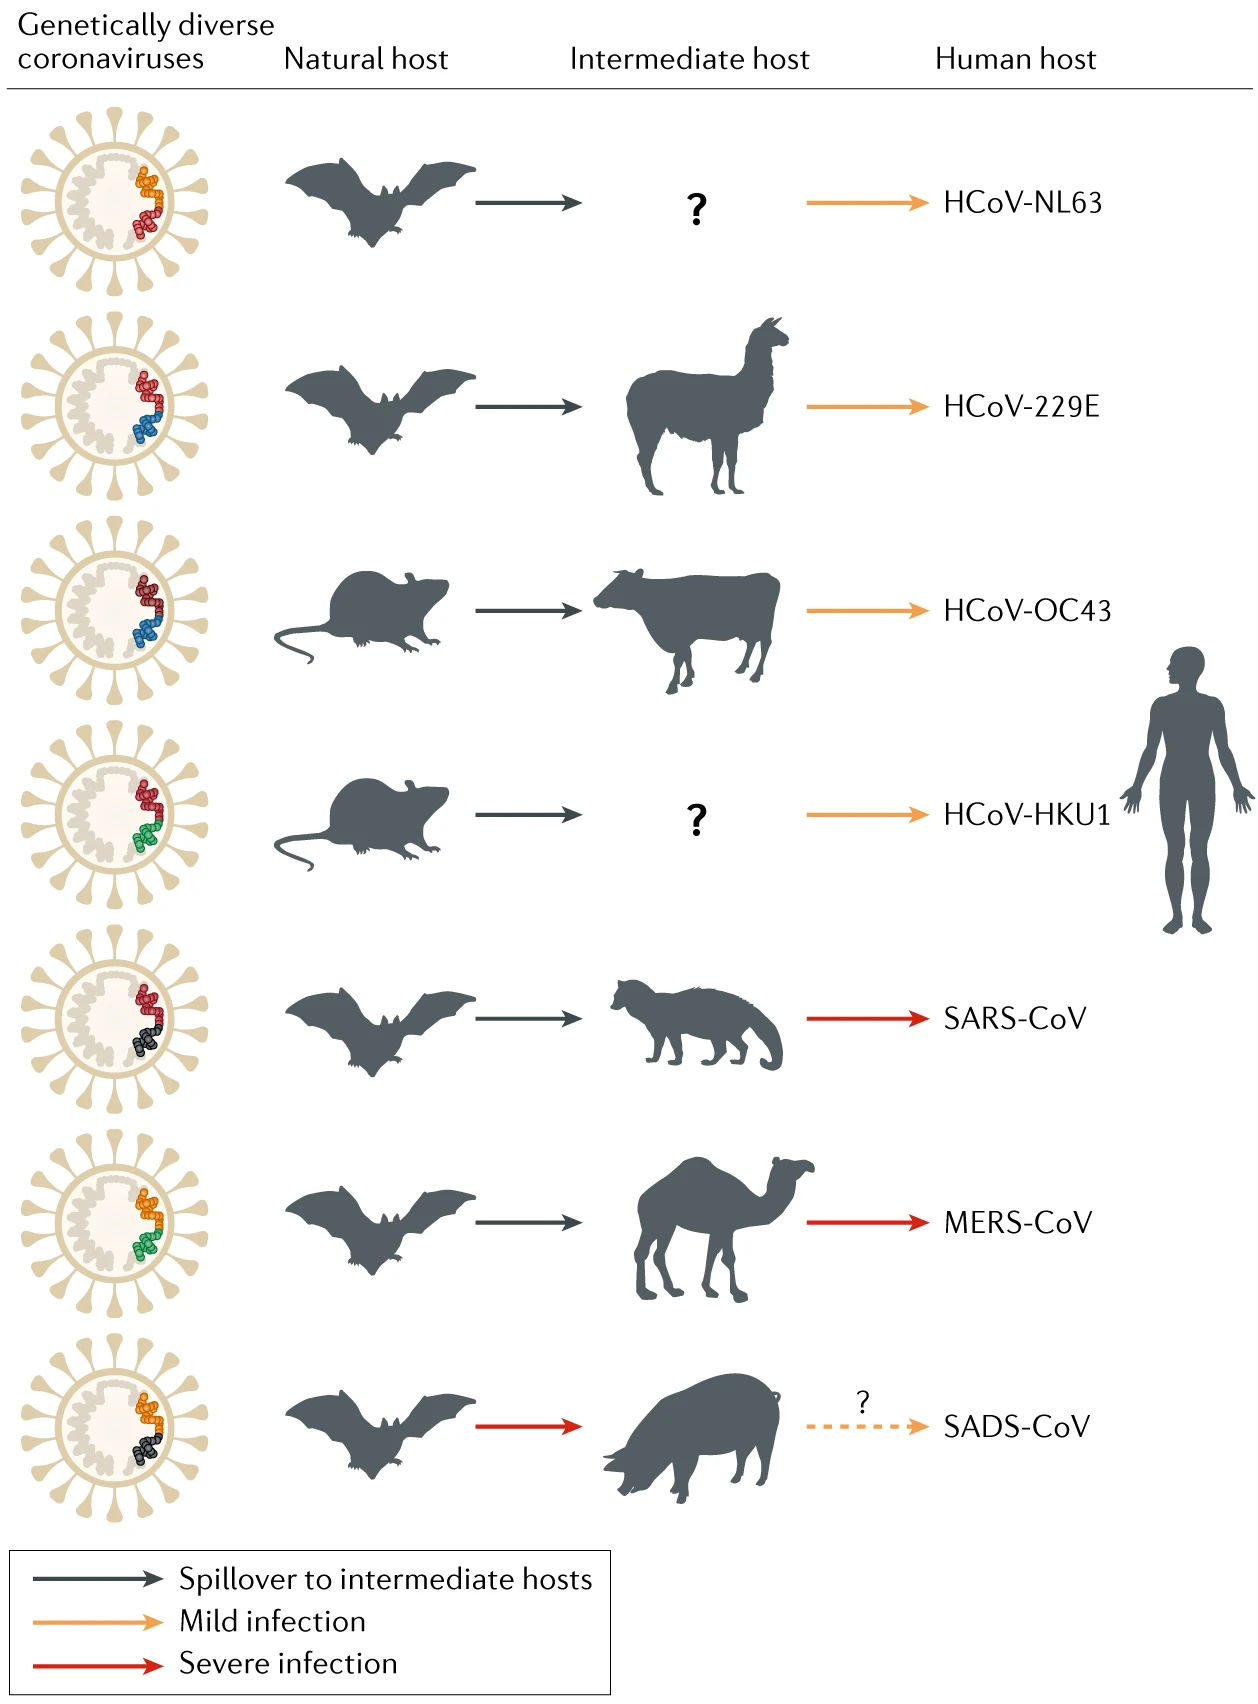
\includegraphics[width=10cm]{img/origin.png} \\
    {\footnotesize \textbf{Fonte: }\cite{cui2019origin}}
    \label{fig:origin}
\end{figure}

\hypertarget{sars-cov-2}{%
\subsection{SARS-CoV-2}\label{sars-cov-2}}

Segundo o autor \cite{de1998epidemia} a palavra endemia significa a ocorrência
de um grande número de casos, uma doença, em um curto período de
tempo. O significado da palavra pandemia tem origem grega dos prefixos neutro
\emph{pan (todo, tudo)} e \emph{demos (povo, população)}. Uma definição moderna é que uma
pandemia é uma epidemia em grande escala que atinge um grande espaço
territorial, como por exemplo diversos países ou o mundo. Mundialmente já
houveram algumas pandemias como gripe espanhola, gripe suína, HIV
e a que estamos enfrentando agora, do vírus SARS-CoV-2 denominado por COVID-19,
que poderá se tornar a maior da história.

De acordo com \cite{guarner2020three} na data de 30 de dezembro de 2019, em
Wuhan, China, houve um relato à Organização Mundial de Saúde (OMS) pelo governo
Chinês de um grupo de pacientes com pneumonia de origem desconhecida. Em 7 de
janeiro de 2020 foi isolado um novo coronavírus destes pacientes, denominado
inicialmente de novo coronavírus 2019 (2019-nCoV), posteriormente tendo o nome
oficializado pela OMS como COVID-19 (SARS-CoV-2.) em 11 de fevereiro de 2020. Os
sintomas deste vírus, assim como o SARS-CoV, são parecidos com a de uma gripe
comum: febre, tosse seca, falta de ar e em casos mais graves, pneumonia. O autor
do artigo \cite{qing2020possibility} cita que a transmissão do COVID-19 ainda
não é totalmente clara, mas já há a confirmação que é, especialmente, através de
gotículas respiratórias e contato direto. Orientações da \cite{covid19OMS} para
prevenção da COVID-19 retirada do seu site:

\begin{itemize}
\tightlist
\item
  Manter distância mínima de 1 metro de outras pessoas.
\item
  Utilizar máscara.
\item
  Limpar as mãos antes de colocar e retirar a máscara.
\item
  Conferir se a máscara cobre o nariz, a boca e o queixo.
\item
  Limpar regularmente, e com atenção, as mãos com um produto à base de álcool ou
  lavá-las com água e sabão.
\item
  Evitar tocar os olhos, nariz e boca.
\item
  Limpar e desinfetar as superfícies com frequência, especialmente aquelas que
  são tocadas de forma regular.
\item
  Evitar ambientes fechados ou cheios.
\item
  Evitar sair de casa.
\end{itemize}

Se você apresentar alguns dos sintomas é recomendável se isolar, e em casos de
presença de febre, tosse e dificuldade de respirar, é indicado procurar
atendimento médico imediatamente. Primeiramente ligue por telefone se puder e
siga as instruções da autoridade de saúde local.

\hypertarget{uxedndice-de-desenvolvimento-humano}{%
\subsection{Índice de Desenvolvimento Humano}\label{uxedndice-de-desenvolvimento-humano}}

\hypertarget{objetivos}{%
\subsection{Objetivos}\label{objetivos}}

\hypertarget{estrutura-de-trabalho}{%
\subsection{Estrutura de Trabalho}\label{estrutura-de-trabalho}}

\hypertarget{MateriaisMetodos}{%
\section{Materiais e Métodos}\label{MateriaisMetodos}}

\hypertarget{shiny}{%
\subsection{Shiny}\label{shiny}}

\hypertarget{Resultados}{%
\section{Resultados}\label{Resultados}}

\nocite{*}

  \bibliography{ic.bib,packages.bib}

\hypertarget{appendix-appendix}{%
\appendix}


\hypertarget{primeiro-apuxeandice}{%
\section{Primeiro Apêndice}\label{primeiro-apuxeandice}}

Este é so um exemplo de Apêndice.

\hypertarget{segundo-apuxeandice}{%
\section{Segundo Apêndice}\label{segundo-apuxeandice}}

Este é so mais um exemplo de Apêndice.

\end{document}
